\documentclass[a4paper]{article}

\usepackage[russian]{babel}
\usepackage[utf8x]{inputenc}
\usepackage{graphicx}
\usepackage{float}
\usepackage{fancyhdr}
\renewcommand{\labelenumii}{\arabic{enumi}.\arabic{enumii}.}

\pagestyle{fancy}
\lfoot{Санкт-Петербургский Губернаторский Физико-Математический Лицей ФМЛ №30}
\renewcommand{\headrulewidth}{0pt}
\rhead{}
\renewcommand{\footrulewidth}{0.4pt}
\rfoot{\thepage}
\cfoot{}

\begin{document}
\begin{titlepage}
\center \Large \textbf{Летняя учебно-исследоватльская практика 2016года}\\
\vspace{2cm}
Группа №16. "ФМЛ №30 Web программирование".\\
\vspace{0.5 cm}

\includegraphics[width=0.5\textwidth]{web_logo.eps}\\
\vspace{0.5 cm}
\textsl{Осипов Глеб}\\
$10^4$-класс ГФМЛ №30

\vspace{7.6 cm}
Санкт-Петербург \\
1-17 июня 2016 года
\end{titlepage}
%\begin{Large}

\section{Введение}
Летняя учебно-исследовательская практика была посвящена изучению основ WEB программирования и проходила в Физико-Математическом Лицей № 30
Computer Science Department в период с 1 июня 2016 года по 17 июня 2016 года.
Изучены темы:
\begin{itemize}
\item Работа с CGI скриптами;
\item Работа с языком програмиррования PHP;
\item Работа с СУБД PostgresSQL;
\item Работа с CSS.
\end{itemize}
\section{Задача и способы ее решения}
\begin{enumerate}

\item \textbf{Постановка задачи}\\
Создание ограниченого доступа к сайту с таблицей умножения.
\item \textbf{Способы решений}
\begin{itemize} 
\item \textit{Использование статичных страниц}\\
Это самый быстрый способ отобржения но он не дает возиожность обрабатывать данные, а соответственно создавать ограниченный доступ.
\item \textit{Использование CGI скриптов}\\
Один из самых быстрых способов отображения и обработки информации, но при этом затрачивается очень много ресурсов сервера, что при большом количестве подключений может повлиять на работоспособность сервера.
\item \textit{Использование интерпретируемых языков программирования}\\
Этот метод реализации задачи требует меньше ресурсов от сервера но при этом работает дольше, чем CGI скрипты, но позволяет реализовать ограниченный доступ к сайту.
\end{itemize} 
\item \textbf{Описание решения}\\
Наша группа реализовывала поставленную задачу, используя \textsl{интерпретируемые языки программирования}, из-за его свойств, отличающих его от остальных методов.\\
\begin{tabular}{c}
\begin{minipage}{\textwidth}
\begin{figure}[H]
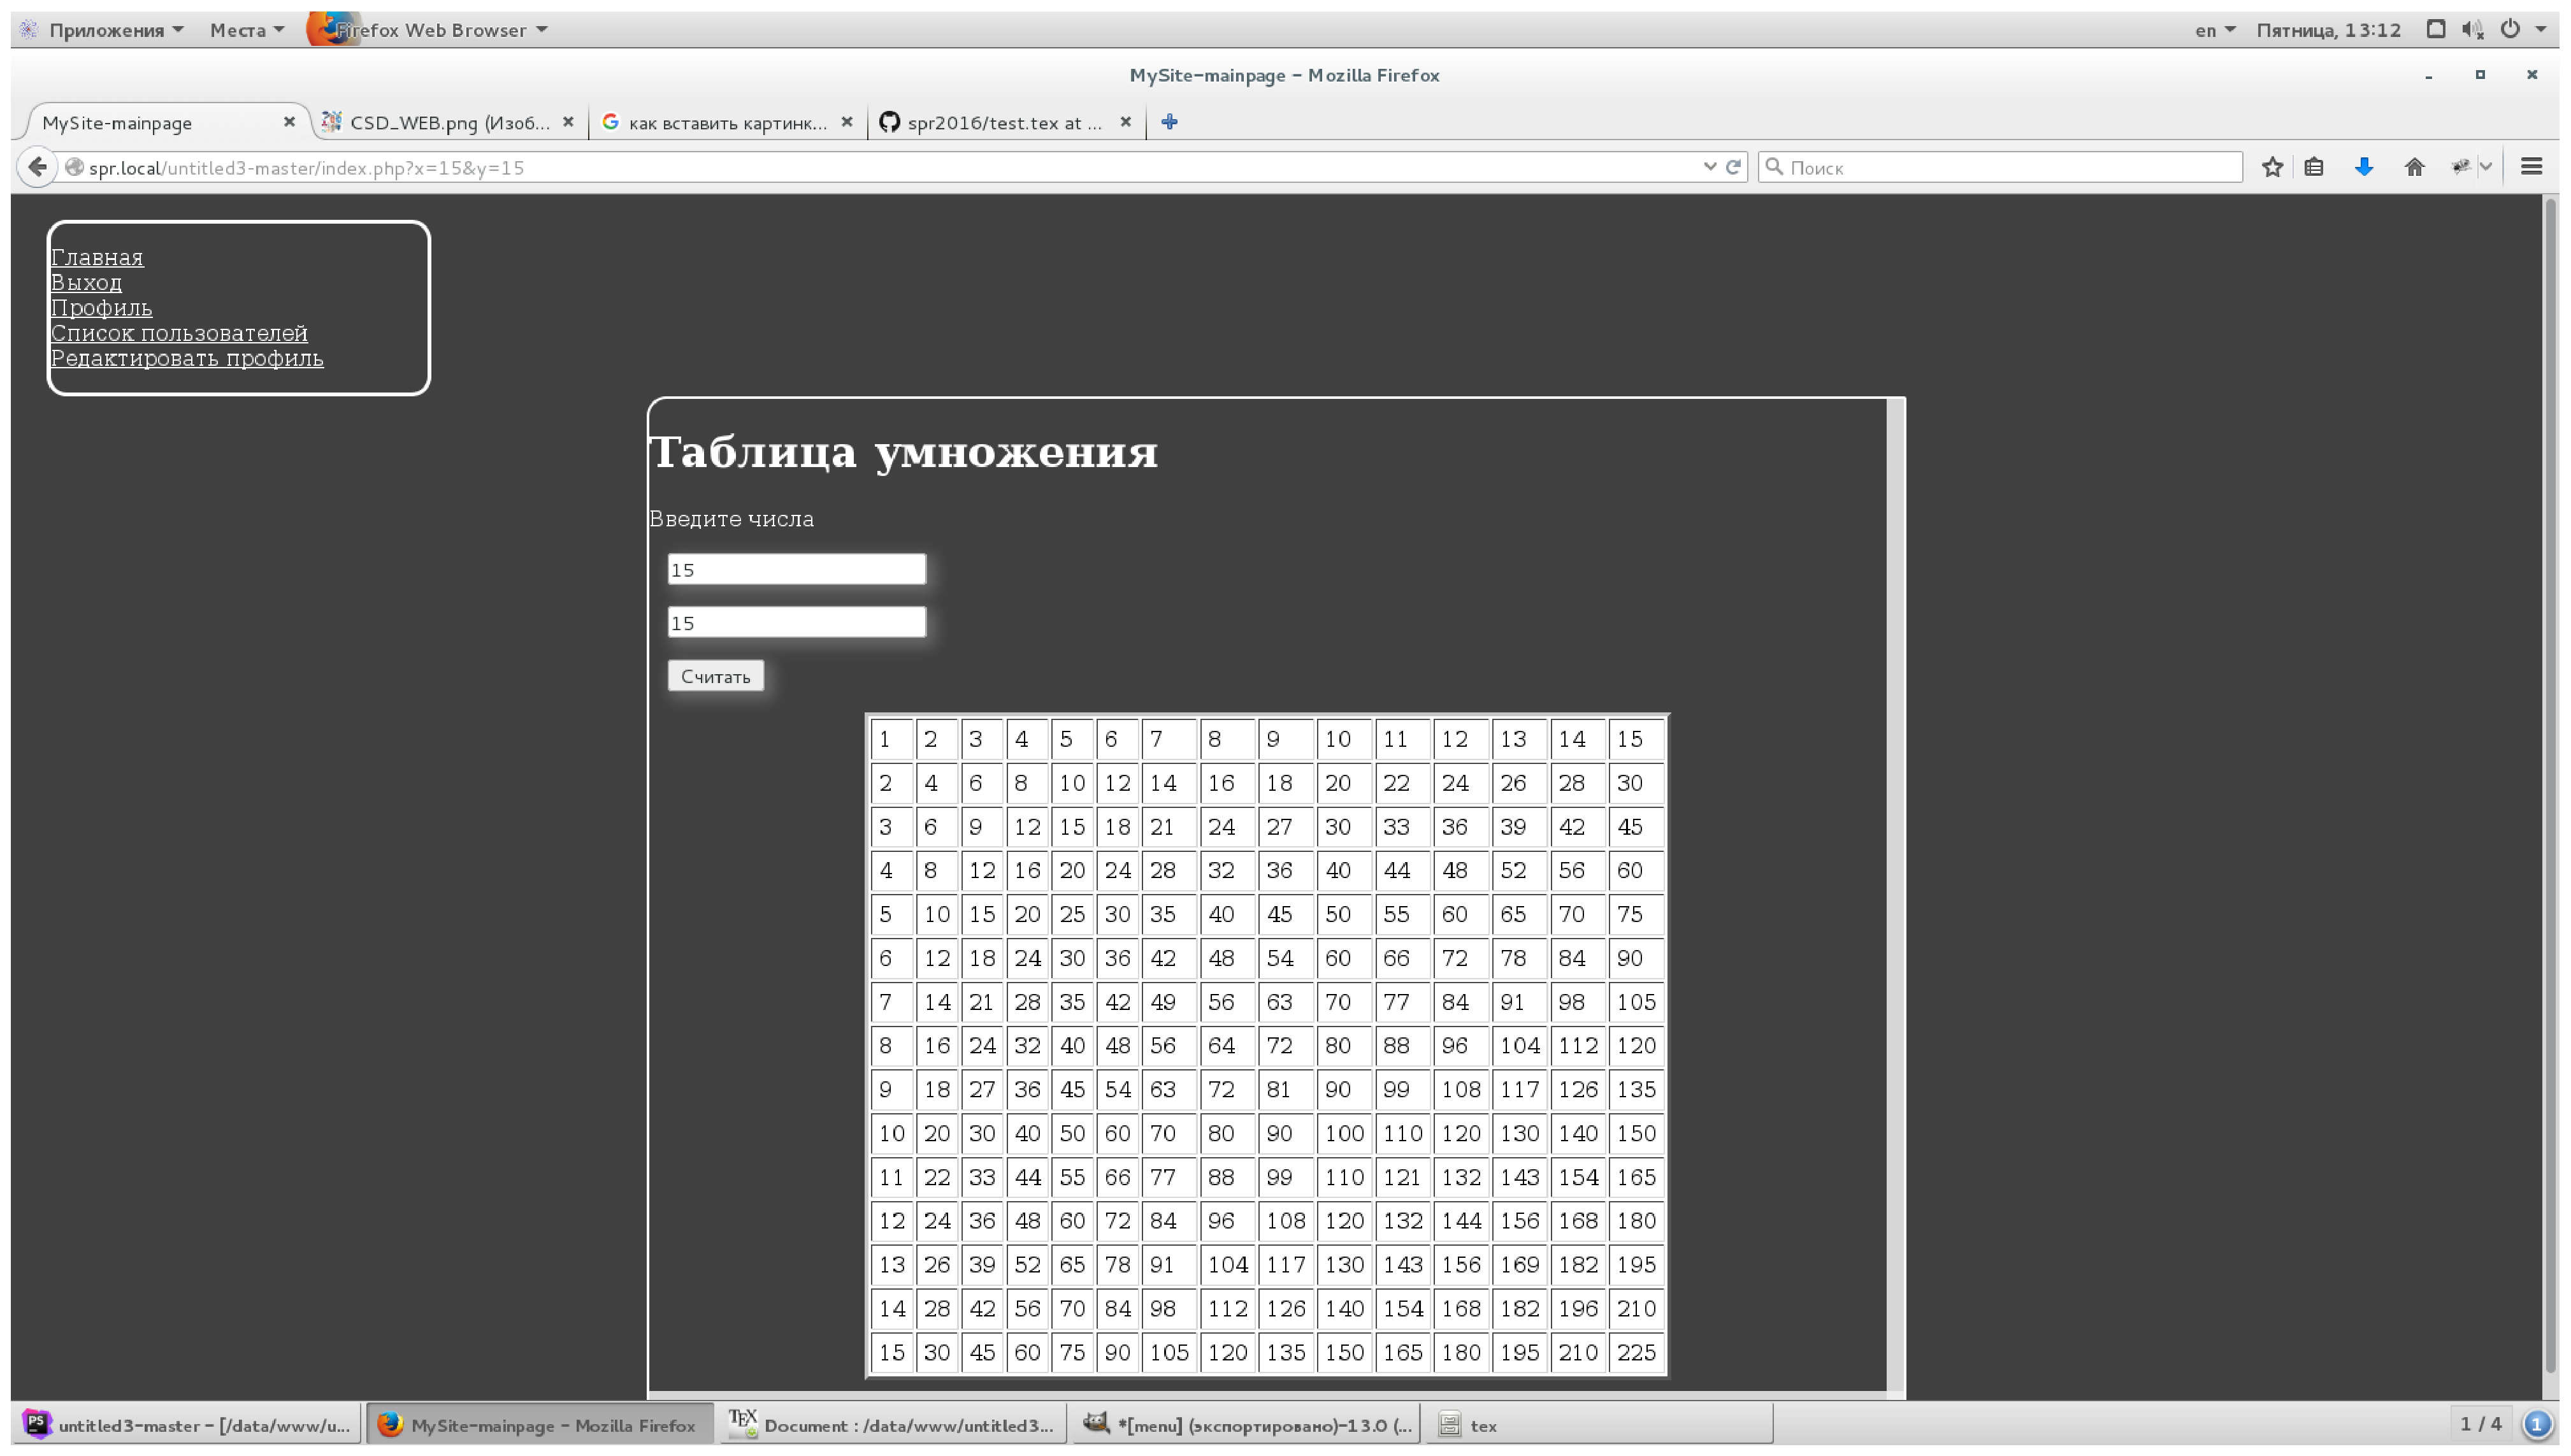
\includegraphics[width=0.63\textwidth]{first_page}
\caption{Вывод таблицы для авторизованного полоьзователя}
\end{figure}
\end{minipage}
\end{tabular}
\textbf{Классы}\\Главной идеей в разработке проекта было отделение отображения от обработки информации, поскольку так намного легче развивать проект, поддерживать егорабочее состояние, а так же для стороннего лица так легче понимать как работает программа и какое действие и где происходит, поэтому были использованы классы \textsl{HTML, USERS, DB(database), SESSION, MENU и HELPERS}, которые подключались из корневых файлов, в которых в зависимости от разных условий подключались бы разные отображения.

\begin{itemize} 
\item \textbf{Класс HTML}\\ 
Главной задачей этого класса была инициализация всех файлов отображения названия которыех были переданы из корневого файла.\\ \textsl{Принцип действия:} в корневом файле вызван калсс HTML в который передается название файла отображения или скрипта(java.script, css)которое нужно подключить, затем  функция template создает массив и переданных названий, впоследствие функция flush подключает все подключенные файлы отображения с нужными параметрами в нужном порядке.
\begin{small}
\begin{verbatim}  
    static public function flush()
    {
        foreach (HTML::$templates as $t) {
            list($name, $args, $type) = $t;
            if ($type != TYPE_META)
                continue;
            include(HTML::$templates_dir . $name . ".php");
        }
        foreach (HTML::$templates as $t) {
            list($name, $args, $type) = $t;
            if ($type == TYPE_META)
                continue;
            include(HTML::$templates_dir . $name . ".php");
        }
    }
\end{verbatim}
\end{small}
\item \textbf{Класс HELPERS}\\
Этот класс отвечает за функции которые были бы полезны в испльзование в каждой из частей WEB сайта, но при этом не отвечающих за какое-то из действий, которые должны выполнять другие классы. Для выполнения данного проекта нам понадобился всего один "помощник"\---get\_or\_post.\\ \textsl{Принцип действия:} при вызове данного класса, т.е. функции get\_or\_post с именем который мы хотим считать из строки запроса или тела запроса она считывает данные из массива GET или POST из ячейки с ключом совпадает с данным  именем и возвращает данные.
\begin{small}
\begin{verbatim}  
function get_or_post($name, $default = null){
    if (isset($_GET[$name]))
        return $_GET[$name];
    if (isset($_POST[$name]))
        return $_POST[$name];
    return $default;
}
\end{verbatim}
\end{small}
\item \textbf{Класс SESSION}\\
В этом классе прописаны функции которые отвечают за работу сервера с файлами сессий (файлами с информацией о подключения пользователя к серверу(cookie) и данных пользователя) и с временной информацией во время сеанса работы пользователя с WEB сайтом.\\ \textsl{Принцип действия:} после того как сервер переда пользователю cookie он сохраняет ее в имя файла, а в последствие использует ее для для поиска данного пользователя. 
\begin{small}
\begin{verbatim}  
static public function start_session()
    {
        Session::$session_started = true;
        if (isset($_COOKIE[Session::$cookie_name]))
            Session::restore_session();
        else
        {
            Session::$uid = md5(microtime(true));
            setcookie(Session::$cookie_name, Session::$uid);
        }
    }
\end{verbatim}
\end{small}
\item \textbf{Класс USERS}\\ 
Данный класс нужен для получения и формирования информации о пользователеях.  Например при регестрации мы можем ввести пароль логин и всю личную информацию, при этом так же мы можем добавить информацию про то какие права у пользователя, что позволит сделать ограниченный доступ к разным отображениям.\\ \textsl{Принцип действия:} этот класс делится на две основные группы функций, которые либо получют парамнетры которые заполнены в базе данных и отдают их пользователю, либо после вызова какой-либо функции из корневого файла с нужными параметрами функция вызывает функции из класса с базами данных и потом по полученым параметрам заполняем нужные поля для пользователя. 
\begin{small}
\begin{verbatim}    
/*Узнает права пользователя. Просто получает пинформацию роль
 пользователя(1группа)*/
    function has_rights($rights)
    {
        return ($this->profile['rights'][$rights] == 't') ?
        true : false;
    }
/*Создание профиля: Получает параметры и создает строку в БД,
а так же заполняет профиль пользователя(2 группа)*/ 
    function create_profile($new_profile)
    {
        global $db;
        if (($res = $db->create_profile($new_profile)['user_create']) > 0)
        {
            $this->authenticated = true;
            $this->profile['login'] = $new_profile['login'];
            $this->profile['password'] = $new_profile['password'];
            $this->set_session();
            return $res;
        }
        return $res;
    }
\end{verbatim}
\end{small}
\item \textbf{Класс DB}\\
Для взаимодействия с СУБД был использован данный класс, главной задачей которого была получить из базы данных информацию и преобразовать и передать для обработки далее.\\ \textsl{Принцип действия:} по полученным параметрам каждая из функций этого класса напрямую работает с базой данных вызывая функцию получая параметры для передачи из пользователю для последующей их обработки.  
\begin{small}
\begin{verbatim}    
/*Функция которая вызывает функцию на языке SQL, для обновления
профиля пользователя в БД*/
    function update_profile($profile)
    {
        return pg_query_params($this->conn, "SELECT * FROM
        update_user($1, $2, $3, $4, $5, $6)",  $profile);
    }
    
/*Функция которая получает все строки таблицы, в каждой из которых
храниться информация про пользователя*/
function all_rows($resource)
    {
        if ($resource === false)
            die("Все плохо: " . pg_last_error($this->conn));
        $res = array();
        while (($row = pg_fetch_assoc($resource)) !== false)
            $res[] = $row;
        return $res;
    }


/*Функция которая получает все строки таблицы*/    
    function one_u($id  = NULL) {
        $resource = pg_query_params($this->conn, "SELECT * FROM
        get_users($1)",
            array($id)) or die(pg_last_error());
        return $this->one_row($resource);
    }
\end{verbatim}
\end{small}
\item \textbf{Класс MENU}\\   
Чтобы пользователю было удобно перемещаться по сайту был создан отдельный класс который выводит карту сайта, с учетом прав пользователя.\\ \textsl{Принцип действия:} при генерации HTML кода будет постоянно вызываться класс MENU в котором выполняться все функции последовательно.  
\begin{small}
\begin{verbatim}    
require_once ("db.php");
class Menu{
    static $map = array(
array("name" => "Главная", "url" => "index.php", "access" => "all"),
array("name" => "Вход", "url" => "sign_in.php", "access" => "guest"),
array("name" => "Выход", "url" => "sign_in.php?function=logout",
"access" => "user"),
array("name" => "Профиль", "url" => "profile.php", "access" => "user"), 
array("name" => "Список пользователей", "url" => "users.php",
"access" => "admin"),
array("name" => "Регестрация", "url" => "sign_up.php",
"access" => "guest"),
array("name" => "Редактировать профиль", 
url" => "profile.php?view=edit", "access" => "user"));
/*Фцнкция создащая HTML код для вывода нужных ссылок для
каждого из пользователей */    
static function get_menu(){
global $user;
    $head_str = "<p>";
    foreach (Menu::$map as $m)
    {
        if ($m['access'] == "all")
            $head_str .= "<a href='" . $m['url'] . "'>" . $m['name'] . "</a><br>";
        elseif ($user->is_auth())
        {
            if ($m['access'] == "user" || ($user->has_rights("users_upd") 
                && $m['access'] == "admin"))
                $head_str .= "<a  href='" . $m['url'] . "'>" . $m['name'] . "</a><br>";
        }
        elseif ($m['access'] == "guest")
            $head_str .= "<a href='" . $m['url'] . "'>" . $m['name'] . "</a><br>";
        }
        $head_str = substr($head_str, 0, strlen($head_str) - 4);
        $head_str .= "</p>";
        return $head_str;
    }
}?>
\end{verbatim}
\end{small}
\begin{tabular}{l}
\begin{minipage}{\textwidth}
\begin{figure}[H]
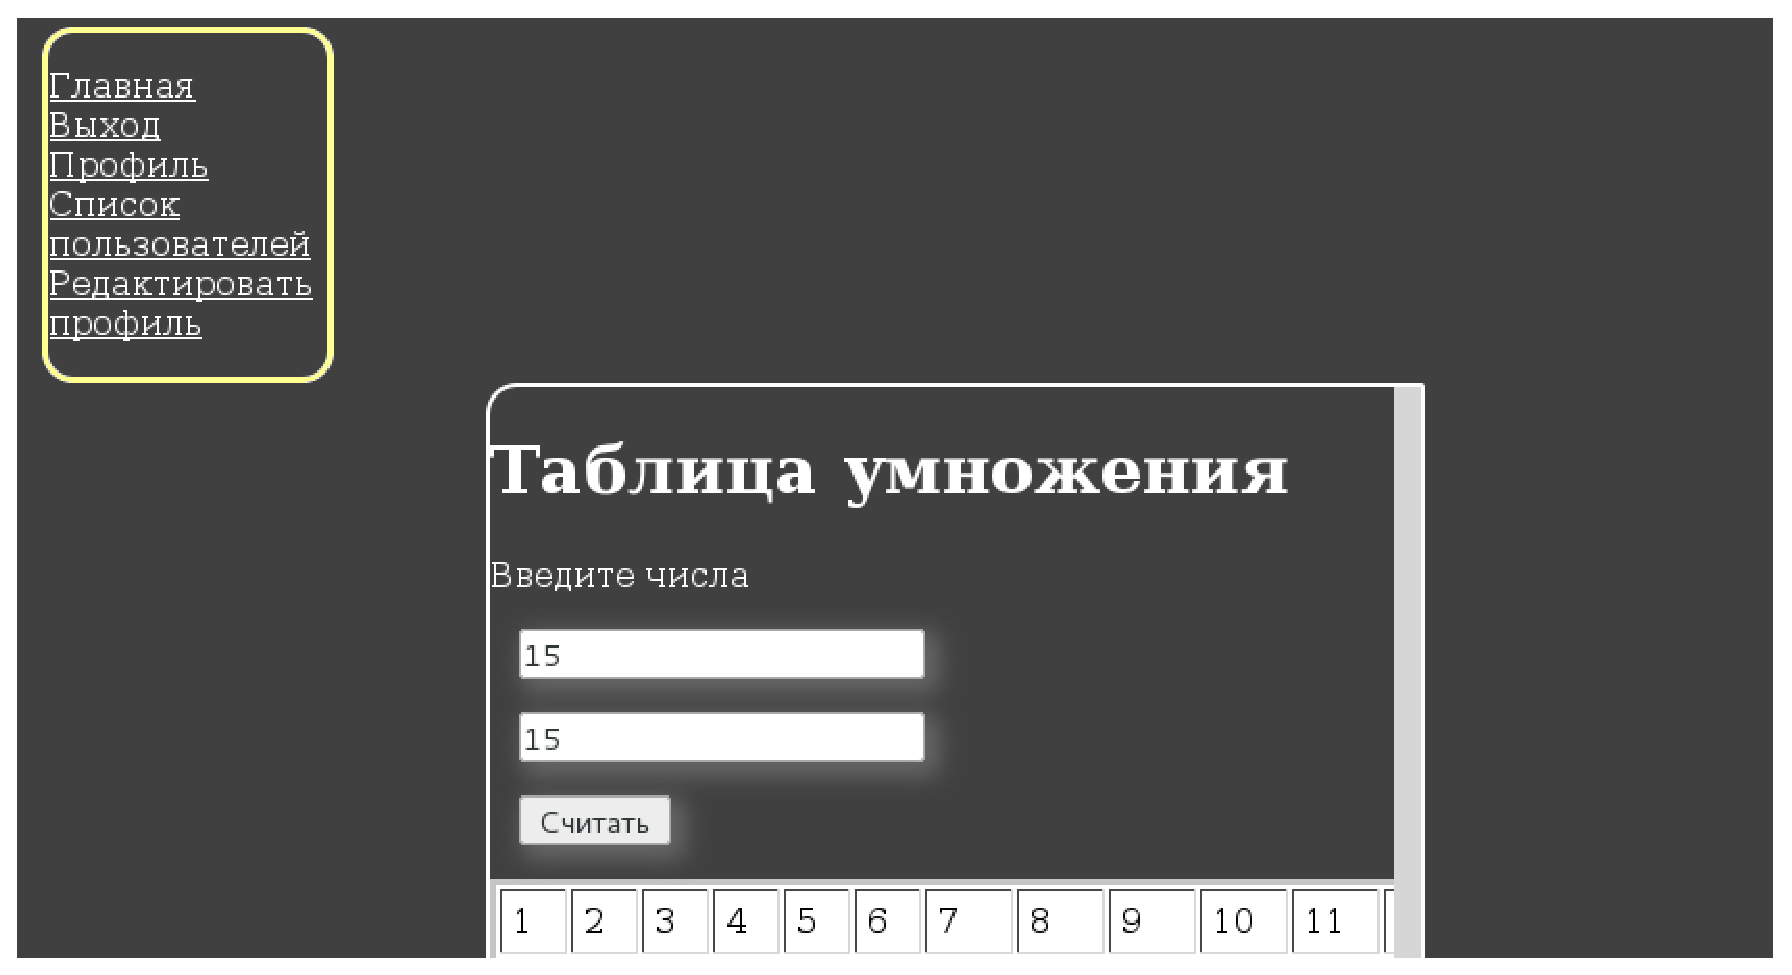
\includegraphics[width=0.5\textwidth]{menu}
\caption{Меню}
\end{figure}
\end{minipage}
\end{tabular}\\

\end{itemize} 

\textbf{Функции базы данных}\\
Так же при реализации этого проекта для работ с базами данных  мы использовали функции написанные на языке SQL. Главной задачей этого метода была ускорить поиск по базе данных, так как построчное считывание очень долгая операция.\\ \textsl{Принцип действия:} в классе DB вызываются SQL функции с заданными параметрами, а фукции выполняют поиск и взвращают таблицу и 

\item \textbf{Вывод}

\end{enumerate}
\section{Заключение}
\section{Используемые программы и материалы}
\end{document}
